\title{Procedurally Generated Indoor Environments for WebGL : Literature Report}
\author{
	Jonathan Frawley \\
	Msc IET \\
	School of Computer Science and Statistics \\
	Trinity College Dublin\\
}
\date{\today}

\documentclass[12pt]{article}

\usepackage{url}
\usepackage{graphicx}
\usepackage{subfig}

\begin{document}
\maketitle

\clearpage

\begin{abstract}
This is a literature review for the Msc in IET programme.
It will outline some of the key resources explored so far in my research and give a state-of-the-art review of the concepts covered.
\end{abstract}

\clearpage

\section{Introduction}
There is an increased interest in recent years in mobile graphics applications and games as well as web graphics.
WebGL presents an opportunity for computer graphics to become accessible to a larger number of users.

\section{Procedural Content Generation}
The generation of procedural content is important for many real-time applications. 
As we will see in this section it has been used to generate vast cities in real-time, the interiors of buildings and graphics effects on standard hardware.
Procedural Content Generation has the potential to 

\subsection{City Generation}
Recently, there has been much interest in the procedural generation of cities.
Ma\"{i}m et al.~\cite{maim2007populating} demonstrated how it is possible to recreate the population of historic cities using procedural techniques.
The use of procedural techniques to generate the crowds in Pompeii allowed realtime simulation with great variety in character representation.
This would not have been possible with traditional techniques.

The Metropolis project~\cite{web:metropolis} investigates the simulation of crowds in a modern city context.
Members of the crowd are modelled based on a variation of some template.
Different clothes are applied to the same templates to give the illusion of variation in the character models~\cite{mcdonnell2007pipeline}.
People are represented as agents which react to their environment~\cite{ulicny2002towards}.
In this way crowds are simulated using a variety of procedural techniques.

\begin{figure}
  \centering
    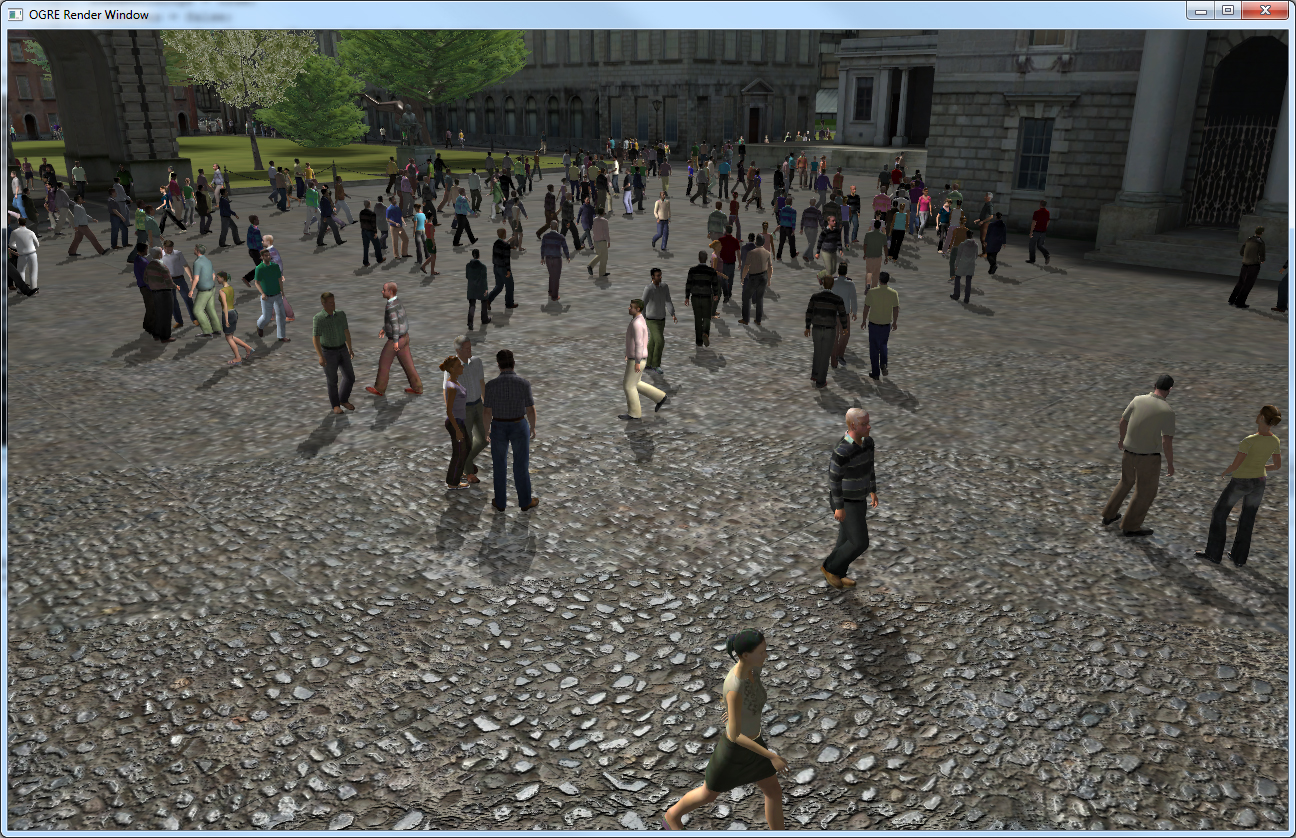
\includegraphics[width=0.7\textwidth]{images/metropolis}
  \caption{Screenshot of the Metropolis program in action}
\end{figure}

CityEngine~\cite{parish2001procedural} is an example of how procedural techniques can be applied to generates environments of great depth.
Using a combination of extended L-systems and self-sensitive L-systems, roads are generated which realistic simulate that of a target city.
Plans of buildings are generated between road segments in a recursive subdivision scheme, which discards inaccessible buildings.
The models of buildings are generated using an L-system using the bounding box of the building as the axiom of the L-system.
A technique known as \emph{layered grids} is proposed for the procedural generation of interesting textures for buildings.

\begin{figure}
  \centering
    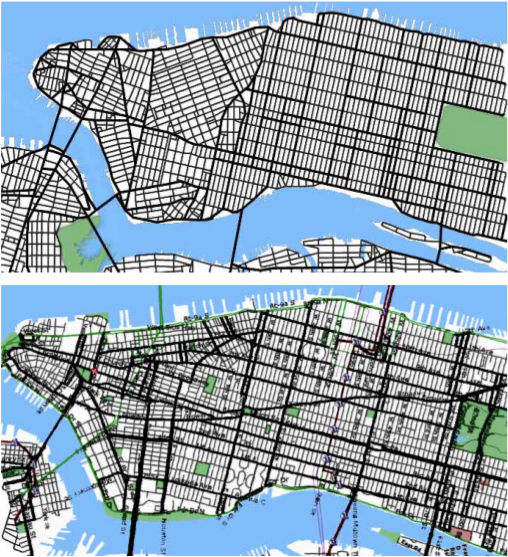
\includegraphics[width=0.7\textwidth]{images/cityengine}
  \caption{Above: Street plan generated by CityEngine. Below: Actual plan of central manhattan.}
\end{figure}


Wonka et. al present a method for automatically modelling architecture~\cite{wonka2003instant} which generates a wide range of architectural features.
A new type of design grammar known as a ``Split grammars'' is used to derive building designs.
This allows the restriction of types of allowed rules. 
These restrictions make the grammars powerful enough for the modelling of buildings.
A parameter matching system allows the user to specify multiple high-level design goals so that the output appears consistent.
Control grammars are introduced which are simple context free grammars which handle spatial ideas in an orderly way which corresponds to architectural principles.
This paper's method gives a useful insight into how architectural features may be used to further enhance the generation of buildings in a procedural way.


\subsection{Building Interiors}
CityEngine provides a method for generating the exteriors of buildings, however this project will focus on the generation of indoor environments using procedural techniques.
Greuter et al. provide methods for generating\cite{greuter2003real} floor plans of buildings in a procedural fashion.
Plans are generated by merging various polygonal shapes in a pseudo-random fashion to generate a final plan of a series of floors.
These floor plans are extruded into the 3rd axes and the outdoor buildings models are created from this.
The floors are not populated with rooms however as the indoor environments are not meant to be seen.

So et al. use wall extrusion for generating 3D indoor environments from floor plans~\cite{so1998reconstruction}.
These generated indoor environments contain rooms.
So et al. apply the technique to a CAD tool, but the technique could easily be applied to an OpenGL-based environment also.

Hahn et al present a novel approach to the generation of virtual building interiors in real-time~\cite{hahn2006persistent}.
The approach uses a lazy generation scheme which is advantageous as it means that the amount of memory used is small. 
They divide the interiors of buildings into temporary regions and built regions.
Built regions contain the final visible product of the generator and hold the geometry needed for collision detection and rendering.
Temporary regions are placeholder regions which are turned into built regions in a lazy fashion.
Temporary regions are populated when the player enters them, via a portal system.
The generation of built regions is split into stages to simplify the implementation:

\begin{enumerate}
	\item Building Setup : Anything which effects multiple floors is generated at this stage. Elevators and stairs are included as well as global textures.
	\item Floor Division : Divides the building into evenly spaced floors. Floors are then divided into 2 parts.
	\item Hallway Division : Hallways are constructed by dividing the regions around other blocks which can be rectangular loops or straight segments of hallway. 
	\item Room Cluster Division : Regions between hallways are divided into rooms. 
	\item Built Region Generation : The geometry of the room is created and it is populated with objects. This is only done if the room contains a portal.
\end{enumerate}

The oldest generated built regions are periodically deleted to control memory. 
Newly generated built regions are put into a LRU cache so that they can be easily recalled if the player moves back into the region.

\section{Demoscene}
The demoscene is a community of computer programmers who specialise in making impressive visual and audio effects.
There is usually an emphasis on small code size such as the 4K competitions which has the restriction on a code size of 4KB~\cite{web:demoscene4k}.
These restricted sized demos are usually referred to as Intros.

Many demoscene programmers have applied their expertise to game-related applications.
One notable example is .theprodukkt~\cite{web:theprodukkt}, who developed the .kkrieger application~\cite{web:kkrieger}.
.kkrieger displays graphics of a level comparable to Doom3 in an executable which is 96K in size.
A comparison of .kkrieger with Doom 3 can be seen in \ref{fig:kkriegerdoomcomp}.
It achieves the results seen using a variety of procedural techniques, many of which will be applicable for this project.
An example is the procedural generation of textures.
It is unfortunant however that Demoscene programmers rarely release the code that they use to produce the effects shown.
This is the case with .kkrieger also.

\begin{figure}
  \centering
  \subfloat[.kkrieger]{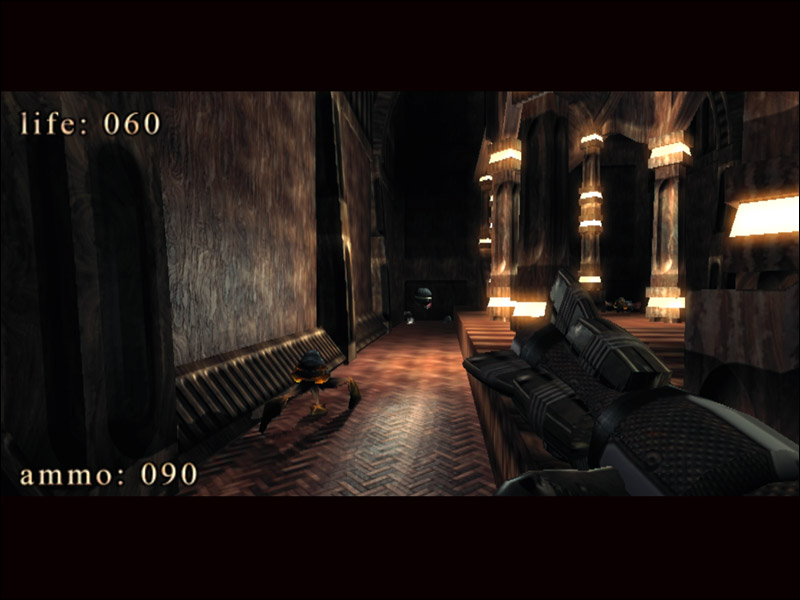
\includegraphics[width=0.5\textwidth]{images/kkrieger}}                
  \subfloat[Doom 3]{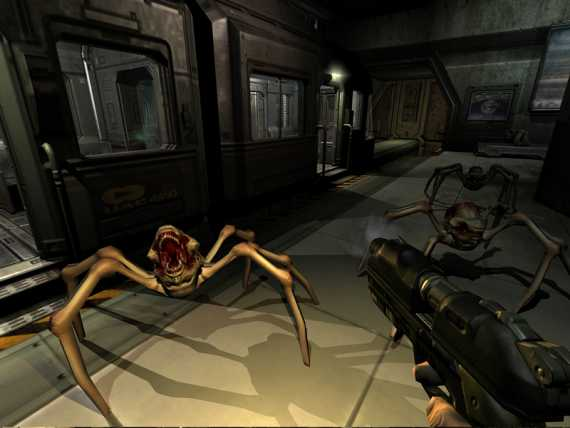
\includegraphics[width=0.5\textwidth]{images/doom3}}                
  \caption{Comparison screenshots of Doom 3 and kkrieger}
  \label{fig:kkriegerdoomcomp}
\end{figure}

\section{WebGL}
WebGL is a draft specification of an API for 3D rendering designed for the web~\cite{web:webglspec}.
It is derived from OpenGL ES 2.0, and provides similar features, within the context of HTML.
WebGL is a rendering context for the HTML5-based canvas element.
WebGL uses GLSL~\cite{web:glsl} language to provide advanced effects such as lighting and texturing.
Since it is based on OpenGL ES 2.0, there are many resources to draw upon when learning how to use it.
There are also many demos already created for WebGL to showcase the functionality~\cite{web:chromeexperiments}.

WebGL is seen by many to be the next step in graphics for web browsers. 
There have been previous attempts to standardise graphics on web browsers such as O3D~\cite{web:o3d} and VRML~\cite{web:vrml}.
WebGL has become the new standard in WebGL and since it is designed by the Khronos group, the same people who standardised OpenGL, people see it as a new era for computer graphics.

\section{Web Frameworks}
There are a variety of web frameworks to choose from nowadays.
This section will discuss a few of them and their merits for use with WebGL.

\paragraph{Javascript}
Javascript is the main language used by web browsers and is built into all modern browsers.
Javascript includes dynamic typing, objects, run-time evaluation.
Functions are first-class objects in javascript, and it is possible to have nested functions.
It uses prototype-based inheritance however, which most programmers would not be familiar with.

There are many quirks in javascript which some programmers abuse and according to Crockford~\cite{web:javascriptbadparts}
It's lack of strong typing and the leniancy of some web browsers on some javascript errors can make it difficult to troublshoot issues.

For use with webgl, the advantage is that javascript is the default language for interacting with webgl.
There are also numerous frameworks written in javascript to ease the use of webgl~\cite{web:threejs}\cite{web:copperlicht}. 

\paragraph{Coffee-script}
Coffee-script~\cite{web:coffeescript} is a language which compiles directly to javascript.
It includes classical inheritance as well as comprehensions and other features which improve upon javascript.
The output javascript passes jslint~\cite{web:jslint}, a javascript code-quality tool.

It also allows the user to use webgl natively and since it compiles to javascript, all of the existing javascript frameworks can easily be used.

\paragraph{Processing.js}
Processing.js~\cite{web:processingjs} is a framework for executing programs written in the Processing~\cite{web:processing} language in the web browser.
Processing is a java-like language for executing small programs known as ``sketches''.
The advantage to processing is that it enables quick demos to be programmed, as a lot of the details of drawing are abstracted away from the programmer.
It has support for WebGL however it does not give the programmer control over the lower-level details of optimisation which may be needed to get maximum performance from this project.

\paragraph{Gwt}
Gwt~\cite{web:gwt} is a framework for creating web applications in Java.
The Java code is compiled to javascript as with Coffee-script.
The advantage to using java is that it is statically typed, is well-known and there are many existing tools to use with it.
The translation is not as straightforward however.
It is also difficult to use javascript libraries with Gwt, requiring the writing of a jsni wrapper~\cite{web:jsni} to communicate back and forth.

There are modules for use with webgl with Gwt.
The most mature of which is gwtgl~\cite{web:gwtgl}.
In testing this out however it is still a work-in-progress and is not stable enough to use for this project.


It was decided to use coffee-script as the language of choice due to it not having some of the weaknesses of javascript, yet having all of its strengths.
This will also be the easiest way to compare the performance against other WebGL implementations as most are written in javascript.

\bibliographystyle{abbrv}
\bibliography{main}

\end{document}
